% TODO:

% Write ``Liquid-vapor interface'' section A.

% Look up question-mark references (citations).

\documentclass[letterpaper,twocolumn,amsmath,amssymb,prb]{revtex4-1}
\usepackage{graphicx}% Include figure files
\usepackage{dcolumn}% Align table columns on decimal point
\usepackage{bm}% bold math
\usepackage{color}
\usepackage{enumitem}

\newcommand{\red}[1]{{\color{red} #1}}
\newcommand{\blue}[1]{{\bf \color{blue} #1}}
\newcommand{\green}[1]{{\bf \color{green} #1}}
\newcommand{\rr}{\textbf{r}}
\newcommand{\kk}{\textbf{k}}
\newcommand{\refnote}{\red{[ref]}}

\newcommand\davidsays[1]{{\bf \color{blue}D: #1}}
\newcommand\kirstiesays[1]{{\bf \color{red}K: #1}}

\newcommand{\fixme}[1]{\red{[#1]}}

\begin{document}
\title{Soft Fundamental Measure Theory Functional for the
  Weeks-Chandler-Anderson Repulsive Potential}

\author{Eric J. Krebs}
\affiliation{Department of Physics, Oregon State University, Corvallis, OR 97331}

\author{Kirstie Finster}
\affiliation{Department of Physics, Oregon State University, Corvallis, OR 97331}

\author{Patrick Kreitzberg}
\affiliation{Department of Physics, Oregon State University, Corvallis, OR 97331}

\author{David Roundy}
\affiliation{Department of Physics, Oregon State University, Corvallis, OR 97331}

%%%%%%%%%%%%%%%%%%%%%%%%%%%%%%%%%%%%%%%%%%%%%%%%%%%%%%%%%%%%
\begin{abstract}
  We introduce an easy-to-implement variation on the Soft Fundamental
  Measure Theory (SFMT) approach for the Weeks-Chandler-Anderson (WCA)
  fluid.  This approach is readily extensible to other soft repulsive
  potentials.  We demonstrate that this approach is comparable in
  accuracy to the Barker-Henderson approach combined with the White
  Bear density functional for the hard-sphere fluid.
\end{abstract}

\maketitle

\subsection{\kirstiesays{Kirstie to-do list}}
\begin{enumerate}
\item Document all the Fourier transforms we are using. (vectors)
\item Find new expressions for alpha and Xi based on virial expansion. (B3)
\item Edit paper to describe/use tensor functional.
\item Write up section on freezing with figures.
\item Decide which equation of state figure to use. (And make pretty.)
\item Touch up the freezing figures.
 
\end{enumerate}

\subsection{Meeting to-do list}
\begin{enumerate}
\item go over plots.
\end{enumerate}

%%%%%%%%%%%%%%%%%%%%%%%%%%%%%%%%%%%%%%%%%%%%%%%%%%%%%%%%%%%%a
\section{Introduction}
The idea of liquids as composed of hard spheres dates back over two
millenia~\cite{lucretius}.  In the 20th century, we came to understand
atoms as inherently soft, but it was shown that their repulsion could
still be accurately described using a hard-sphere model, provided the
radius is chosen to be temperature
dependent~\cite{rowlinson1964statistical, barker1967perturbation,
  andersen1971relationship}.  These works cemented the hard-sphere
model as the reference system of choice for the theory of
liquids~\cite{gil-villegas-1997-SAFT-VR, clark2006developing,
  lafitte2013accurate}.  The hard-sphere fluid is
widely studied and well understood, not only for the homogeneous
fluid~\cite{carnahan1969equation}, but also in the more challenging
case of the inhomogeneous fluid~\cite{rosenfeld1989, rosenfeld1997,
  roth2002whitebear}.  However, the hard-sphere fluid remains a
non-physical model, which can also be numerically inconvenient due to its
discontinuous potential, and the requirement for delta functions in
computing weighted densities.

Fundamental Measure Theory~(FMT) is a classical density functional
theory for the free energy of the hard-sphere fluid developed by
Rosenfeld~\cite{rosenfeld1989}.  Due to its combination of
computational efficiency with accuracy, FMT has since been used as the
basis for a wide variety of classical density
functionals~\cite{cuesta1997dimensional, hansen2009fundamental,
  marechal2013density, hughes2013classical, krebs2014improved}.
%
In 1999, Schmidt introduced \emph{Soft} Fundamental Measure Theory
(SFMT)~\cite{schmidt1999density}, which directly treats soft repulsive
potentials in a framework based on the highly successful FMT.  SFMT
has been used to describe the behavior of a star polymer in
solution~\cite{schmidt2000density, groh2001density, kim2001adsorption,
  sweatman2002fundamental}, as well as repulsive potentials applicable
to atoms~\cite{schmidt2000fluid, sweatman2002fundamental}.

%% In his 2010 review of FMT, Roth states that the most important future
%% developments in equilibrium DFT will involve treating soft repulsions
%% and attractions~\cite{}.

In this paper, we will apply SFMT to study the Weeks-Chandler-Anderson
(WCA) repulsive potential~\cite{weeks1971}.  This potential reproduces
the repulsive force of a Lennard-Jones interaction, which makes it an
ideal model for interatomic repulsion.  Mathematically, the WCA
pair potential is given by
\newcommand\erf{\mathrm{erf}}
\newcommand\Vwca{V_{\mathrm{wca}}}
\newcommand\Verf{V_{\erf}}
\begin{align}
  \Vwca(r) =
  \begin{cases}
    4\epsilon \left[ \left(\frac{\sigma}{r}\right)^{12} -
    \left(\frac{\sigma}{r}\right)^{6} \right] + \epsilon, & 0 < r < 2R \\
    0, & \textrm{otherwise}.
  \end{cases}
\label{eq:Vwca}
\end{align}
where $\epsilon$ and $\sigma$ are the usual Lennard-Jones parameters
and $R$ is a single sphere radius which is related by $\sigma =
2^{5/6} R$. In this paper we will use the dimensionless reduced
density $n^* \equiv n \sigma^3$ and reduced temperature $T^* \equiv
k_BT/\epsilon$.

\section{Methods}

\subsection{Soft Fundamental Measure Theory}

The excess free energy of SFMT, like that of Rosenfeld's
FMT~\cite{rosenfeld1989}, is derived using dimensional crossover 
from the exact free energy in the zero-dimensional cavity limit~\cite{schmidt1999density}. 
It is written as an integral of functions
\begin{equation}
A_\textit{SFMT}[n] = k_B T \int \left(\Phi_1(\rr) + \Phi_2(\rr) +
\Phi_3(\rr)\right) d\rr \; , \label{eq:sfmt-excess-free}
\end{equation}
with integrands
\begin{align}
\Phi_1 &= -n_0 \ln\left( 1 - n_3\right)\\
\Phi_2 &= \frac{n_1 n_2 - \mathbf{n}_{V1}\cdot\mathbf{n}_{V2}}{1-n_3} \\
%\Phi_3 &= \frac{{n_2}^3-3n_2\mathbf{n}_{V2}\cdot\mathbf{n}_{V2}+\frac{9}{2}[\mathbf{n}_{V2}\cdot{\overleftrightarrow{n}_{m2}}\cdot{\mathbf{n}_{V2}}-\operatorname{Tr}({\overleftrightarrow{n}^3_{m2}})]}{24\pi(1-n_3)^2}\\
\Phi_3 &= \frac{1}{24\pi(1-n_3)^2}\left({n_2}^3-3n_2\mathbf{n}_{V2}\cdot\mathbf{n}_{V2}\color{white}\frac{1}{1}\right)\color{black}
%+\frac{9}{2}[\mathbf{n}_{V2}\cdot{\overleftrightarrow{n}_{m2}}\cdot{\mathbf{n}_{V2}}-\operatorname{Tr}({\overleftrightarrow{n}^3_{m2}})]
\label{eq:sfmt-phi3}
\end{align}
\begin{displaymath}\color{white}\left(\color{black}+\frac{9}{2}[\mathbf{n}_{V2}\cdot{\overleftrightarrow{n}_{m2}}\cdot{\mathbf{n}_{V2}}-\operatorname{Tr}({\overleftrightarrow{n}^3_{m2}})]\right)\end{displaymath}
where we have used the tensor version of $\Phi_3$ formulated by Tarazona~\cite{tarazonaYEAR  phi3,santos2012phi3}.
The integrands are functions of a set of weighted densities $n_{i}(\textbf{r})$ given by %known as \emph{fundamental measures}.
%The integrand functions are functions of a set of weighted densities known as \emph{fundamental measures} derived using dimensional crossover from the exact free energy
%in the zero-dimensional cavity limit~\cite{schmidt1999density}.
%which are functions of a set of weighted densities known as \emph{fundamental measures}, 
%and which are derived using dimensional crossover from the exact free energy
%in the zero-dimensional cavity limit~\cite{schmidt1999density}.
%The fundamental measures
\begin{equation}
  n_{i}(\textbf{r}) = \int
  n(\textbf{r}')w_i(|\textbf{r}-\textbf{r}'|) d\textbf{r}'
  \label{eq:n-convolution}
\end{equation}
are defined as convolutions with weight functions similar to those of
hard-sphere FMT. Like hard-sphere fundamental measures, the new weight
functions are constructed so as to deconvolve the Mayer function,
\begin{equation}
  f(r) = e^{-\beta V(r)} - 1
  \label{eq:Mayerfunction}
\end{equation}
where $\beta = 1/k_BT$. %, which in the case of hard spheres is just a
%step function.  
The weighting functions are related by
\begin{align}
  w_1 &= \frac{w_2}{4\pi r} &
  w_0 &= \frac{w_2}{4\pi r^2}
  \label{eq:n-0-1}
  \\
  \mathbf{w}_{V2} &= w_2\frac{\textbf{r}}{r} &
  \mathbf{w}_{V1} &= w_1\frac{\textbf{r}}{r}
  \label{eq:n-vectors}
\end{align}
\begin{equation}
  \overleftrightarrow{w}_{m2} = w_2(r)\left(\frac{\mathbf{rr}}{r^2}-\frac{I}{3}\right)
  \label{eq:n-tensor}
\end{equation}
\begin{equation}
   w_3(r) = \int_{r}^{\infty} w_2(r') dr',
  \label{eq:n-3}
\end{equation}
where we note that the integral in Eq.~\ref{eq:n-3} is a
one-dimensional integral over radius. Schmidt proved that as in traditional hard-sphere fundamental measure theory, 
SFMT reproduces the exact functional in the low-density limit, provided the 
weighting function that defines $n_2$ is related to the slope of the Mayer 
function by a convolution with itself
\begin{equation}\label{eq:mayerandw2}
  \frac{d f(r)}{dr} = \int dr' w_2(r') w_2 (r-r').
\end{equation}
%with the other weighting functions given by the equations above
%~\cite{schmidt2000fluid}.  
%We note that these equations %---which equations exactly???----
%are satisfied by traditional hard-sphere FMT as well as SFMT, for the same
%reason: they are needed in order to ensure the correct low-density
%behavior.  
%One way of using Equation~\ref{eq:mayerandw2}, would be to choose a pair potential and deconvolve the Mayer
%function to solve for $w_2$. 
%Equation~\ref{eq:mayerandw2} is the challenge point for SFMT:
%There are two options for constructing a theory directly using SFMT:
%%In constructing a theory directly using SFMT, there are two options to consider.
%either one must choose a pair potential and deconvolve the Mayer
%function to solve for $w_2$---which is difficult---or one can
%construct a $w_2$ and solve for the pair potential that weighting
%function represents. 
%However, deconvolving the Mayer $f$ function for a realistic potential is
%From Equations~\ref{eq:Mayerfunction} and \ref{eq:mayerandw2} it can be seen that  

One way to satisfy Equation~\ref{eq:mayerandw2} is to choose a pair potential $V(r)$ and deconvolve the Mayer function $f(r)$ to solve for $w_2(r)$. 
However, deconvolving the Mayer function for a realistic potential is challenging, which has limited the number of applications of this
theory to liquids in which the potential energy of interaction is
proportional to the temperature. 
In the original papers introducing SFMT, Schmidt
exclusively studied models analytically in which the potential is
proportional to temperature~\cite{schmidt1999density,
  schmidt2000fluid}.  While this proportionality is correct for purely
entropic interactions, such as the star polymer in solution studied in
several papers~\cite{schmidt1999density}, this assumption is not
applicable to energetic interactions such as dominate the repulsion
between molecules.

Alternatively, one can 
construct a $w_2(r)$, and use Equation~\ref{eq:mayerandw2} to solve for the pair potential that weighting
function represents.  
%In this paper, we will 
%This is the approach we use in this paper.
This is the approach we use in this paper. We use a weighting function for $w_2(r)$ introduced by Schmidt in Ref.~\citenum{schmidt2000fluid} which has the form of a Gaussian 
%is formed using the analytically simple \emph{error function model} (or \emph{erf model}) introduced by Schmidt in 
%Ref.~\citenum{schmidt2000fluid}.
%which is a analytically simple functional form.  
%In the erf model, the weighting function $w_2$ has the form of a Gaussian %The erf model corresponds to a Gaussian form for the
%weighting function $w_2$:
\begin{align}
  w_2(r) &= \frac{\sqrt{2}}{\Xi \sqrt{\pi}} e^{-\left( \frac{r-\alpha/2}{\frac{\Xi}{\sqrt{2}}} \right)^2}
  \label{eq:gaussianw2}
\end{align}
where $\Xi$ and $\alpha$ are parameters with dimensions of length.
This choice for $w_2(r)$ results in analytically simple forms 
for the $w_3(r)$ weighting function, the Mayer function, and the pair
potential where each contains an error function:
\begin{align}
  w_3(r) &= \tfrac12 \left( 1 - \mathrm{erf}\left(\frac{r-\alpha/2}{\frac{\Xi}{\sqrt{2}}}\right) \right) \\
  f(r) &= \tfrac12 \left( \mathrm{erf}\left( \frac{r - \alpha}{\Xi} \right) - 1 \right)
  \label{eq:mayer-approx} \\
  \Verf(r) &= -kT\ln\left[\tfrac12 \left( \mathrm{erf}\left( \frac{r -
    \alpha}{\Xi} \right) + 1 \right) \right].\label{eq:Verf}
\end{align}
This model is called the \emph{error function model} (or \emph{erf model}). The erf potential is shown in Fig.~\ref{fig:potential-plot}, and the
first derivative of the Mayer $f$ function corresponding to this
potential is shown in Fig.~\ref{fig:w2-comparison}.  

Fourier transforms of the weight functions are used to solve for the weighted densities in Equation~\ref{eq:n-convolution}.  Analytical expressions for the Fourier transforms of each of the weighting functions is provided in Appendix~\ref{sec:fourier}.
\subsection{Soft FMT for the WCA fluid}

\begin{figure}
\begin{center}
\includegraphics[width=\columnwidth]{figs/potential-plot}
\end{center}
\caption{The WCA potential, and approximations to this potential
  constructed for two different temperatures.}
\label{fig:potential-plot}
\end{figure}

%Our approach is to approximate the effect a soft repulsive potential
%%(specifically the potential of the WCA fluid) by using the erf
%potential with temperature-dependent parameters.  
%We select the
%parameter $\alpha$ to match the value 
%and derivative of
%$\Verf(r)$ and $\Vwca(r)$ at the distance $\alpha$, corresponding to
%the maximum slope of the Mayer $f$ function.  (Thus, we are using the
%erf potential in the same way that the Barker-Henderson approach uses
%the hard-sphere potential to model a soft repulsive fluid.)

\begin{figure}
\begin{center}
\includegraphics[width=\columnwidth]{figs/w2-comparison}
\end{center}
\caption{The derivative of the Mayer function $f(r)$ from the WCA
  potential, and the convolution of the fitted Gaussian $w_2$ with
  itself at two different temperatures.  According to
  Eq.~\ref{eq:mayerandw2} these should be identical in order to
  accurately reproduce the low-density behavior of the fluid.}
\label{fig:w2-comparison}
\end{figure}

%As is evident
%from Eq.~\ref{eq:Verf}, if the potential energy of interaction is
%temperature-independent, then this simple form for $w_2(r)$ can only hold
%for one temperature.  At other temperatures, the same potential leads
%to an entirely different form for $f(r)$ and $w_2(r)$, which is not
%analytically tractable.

%Our approach is to 
We approximate the effect of a soft repulsive potential
(specifically the potential of the WCA fluid) by using the erf
potential. However, as is evident
from Eq.~\ref{eq:Verf}, if the potential energy of interaction is
temperature-independent, then this simple form for $w_2(r)$ can only hold
for one temperature.  At other temperatures, the same potential leads
to an entirely different form for $f(r)$ and $w_2(r)$, which is not
analytically tractable.

Our approach is to use the erf potential with temperature-dependent parameters. 
We begin by equating the values of the potentials $\Verf(r)$ and $\Vwca(r)$ at distance
$\alpha$ corresponding to
the maximum slope of the Mayer function. This tells us that the $\alpha$ parameter must be given by
\begin{align}
  \alpha = \sigma \left( \frac{2}{1 + \sqrt{\frac{k_BT}{\epsilon}
        \ln 2}} \right)^{\frac{1}{6}}.
\end{align}
The alpha parameter roughly measures the length-scale of the
interaction, and like the Barker-Henderson diameter discussed later, decreases with
increasing temperature.  Next, we set the second virial coeffecient formed using 
the mayer function for the $\Vwca(r)$ potential in Eq.~\ref{eq:Vwca} equal to the second virial coefficent formed using the mayer function for the $\Verf(r)$ potential in Eq.~\ref{eq:Verf}, and solve for the parameter $\Xi$ at a given temperature.
%\begin{displaymath}B_2=-\frac{1}{2}\int{f(r)~d{r}}\end{displaymath}
\begin{equation}B_2=-\frac{1}{2}\int{(e^{-\beta V(r)} - 1)~d{\vec{r}}}\end{equation}
%\begin{displaymath}\int{(e^{-\beta V_{wca}(r)} - 1)~d{r}}=\int{(e^{-\beta V_{erf}(r)} - 1)~d{r}}\end{displaymath}
%Finally, equating the slope of both
%potentials at $r = \alpha$ yields the other parameter
%\begin{align}
%  \Xi = \frac{\alpha}{6\sqrt{\pi} \left( \sqrt{\frac{\epsilon}{k_BT} \ln
%      2} + \ln 2 \right)},
%\end{align}
The Xi parameter is a measure of the effective softness of the interaction, and
increases with the temperature.  

We show the resulting approximation
for the potential in Figures~\ref{fig:potential-plot} for two
different temperatures.  We see the temperature dependence of the
approximation in comparison to the WCA potential, with the
approximation at higher temperatures being more accurate for smaller
differences. Vertical dotted lines show the values of $\alpha$ at
which $\Verf$ and $\Vwca$ are matched, a solid black vertical line
represents the distance at which the WCA force goes to zero, and the
horizontal dotted lines illustrate the two temperatures.  At both
temperatures, the largest deviations are seen at very small distances,
and thus very high potential energies.

Figure~\ref{fig:w2-comparison} compares the derivative of the Mayer
function corresponding to the WCA pair potential with convolution of
the the fitted Gaussian $w_2$ from Eq.~\ref{eq:gaussianw2} with
itself, as in Eq.~\ref{eq:mayerandw2}.  \color{red}The two vertical dotted lines
show the $\alpha$ where the potential functions have been matched, and
the the solid vertical line shows where the WCA force, and potential,
and thus $f'_{\mathrm{wca}}$, goes to zero. The erf result extends
slightly past the cutoff at which $f'_{\mathrm{wca}}$ vanishes for
both temperatures, but does quickly go to zero. At lower lower
temperatures $w_2$ and $f'$ are more peaked and approach the cutoff, as
the system approaches hard-sphere behavior in which these functions
are Dirac $\delta$ functions.\color{black} 

%In this step, we make one additional approximation beyond the erf
%approximation, which is to approximate $w_0$ as a linear combination
%of $w_1$ and $w_2$, which results from a power series approximation
%valid in the low-temperature limit, when $\Xi\ll\alpha$.

\subsection{Freezing of the WCA fluid}

Freezing is governed by entropy which the universe, or any closed system, seeks to maximize according to the second law of Thermodynamics. When the entropy of a pure substance in its liquid state is lower than the entropy that it would have in its solid state at the same temperature, pressure, and chemical potential an abrupt phase transistion occurs, that is, the liquid freezes forming a crystalline structure. The particular crystalline structure and density that result are affected by the interatomic potential. When the soft sphere WCA fluid freezes, a Face Centered Cubic (FCC) lattice is formed~\cite{reference!} with a total of one atom in each parallelpiped-shaped primative cell. 

The equilibrium Helmholtz free energy of the crystal, and its corresponding equilibrium number density profile $n(\vec{r})$ can be found at a given temperature simply by varying the number density spatially 
%, the spatially varying number density, 
%by changing %the spatial profile of the number density by varying 
%the width of the gaussians centered at each lattice point, and the crystal cell size 
until the free energy
% - which is a functional of $n(\vec{r})$ - 
is minimized. For the crystal the $n(\vec{r})$ used in the integral in Eq.\ref{eq:n-convolution} is given by Gaussians centered at each lattice point specified by $\vec{R_i}$. 
\begin{equation}n(\textbf{r})= \frac{1}{\left(\sqrt{2\pi}\sigma_{g}\right)^3}\int{e^{-\frac{|\vec{r}-\vec{R}|^2}{2\left(\sigma_g\right)^2}}d{\vec{r}}}  \end{equation}  
$n(\vec{r})$ is changed by varying the width of the gaussians, \color{red} and by changing the size of the crystal cell. \color{black}As the gaussian width gets large, the number density becomes homogeneous. \color{red}A larger crystal cell models a larger fraction of vacancies. \color{black} Monte-Carlo integration is employed to more efficiently compute the weighted densities used to calculate the excess free energy which is then added to the ideal free energy (computed analytically) to get the total free energy which is minimized. The pressure is found from the negative of the slope of the Helmholtz free energy per atom with respect to the inverse number density. \begin{equation}{P=-\frac{\partial{\frac{F}{N}}}{\partial{\frac{V}{N}}}\bigg|_{T,N} = -\frac{\partial{f}}{\partial{\frac{1}{n}}}\bigg|_{T,N}}\end{equation} 
The densities of both the solid and the liquid at the solid-liquid transition can then be found using Maxwell's double tangent construction which equates the pressure of the fluid and of the solid at the phase transition.




\subsection{Comparison to Barker-Henderson hard sphere}

%Another approach to account for the temperature dependence of
%realistic fluids is Barker-Henderson's
%approach~\cite{barker1967perturbation}. This theory takes any general
The Barker-Henderson fluid is known to give good results, so we use it as a reference to compare with our DFT results. 
In the BH approach, any general
repulsive pair potential, $V(r)$ is used to construct a corresponding hard
sphere reference fluid with a temperature dependent diameter. The hard
sphere diameter is given by
\begin{align}
  d = \int_0^{\infty}\left( 1 - e^{-\beta V(r)} \right)\mathrm{dr}.
  \label{eq:bh-diameter}
\end{align}
We utilize this variable diameter with the White Bear FMT free energy
functional for the hard sphere fluid~\cite{roth2002whitebear} as a
comparison for the SFMT presented in this paper.

The White Bear version of the Fundamental-Measure Theory~(FMT)
functional~\cite{roth2002whitebear}, \color{red}describes the excess free energy
of an \emph{inhomogeneous} hard-sphere fluid.  This functional differs
from the equations of SFMT presented in
Equations~\ref{eq:sfmt-excess-free}-\ref{eq:n-3} only in replacing
Eq.~\ref{eq:sfmt-phi3} with the following equation:
\begin{align}
\Phi_3 &= (n_2^3 - 3 n_2 \mathbf{n}_{V2} \cdot \mathbf{n}_{V2}) \frac{
  n_3 + (1-n_3)^2 \ln(1-n_3)
}{
  36\pi n_3^2\left( 1 - n_3 \right)^2
} ,
\end{align}
which causes the functional to reduce to the Carnahan-Starling free
energy rather than scaled-particle theory for homogeneous systems. \color{black} In
addition, the weighting function $w_2$ for a hard-sphere system is
given by the Dirac $\delta$ function:
\begin{align}
  w_2(r) = \delta(r - R),
\end{align}
where $R$ is the hard-sphere radius.  The remaining weighting
functions are derived from $w_2$ according to
Eqs.~\ref{eq:n-0-1}-\ref{eq:n-3}, as in SFMT.






\section{Results}
In this section the results of our SFMT method will be compared to the results of simulations for a reference fluid.
For all of our reference simulations, we construct a Barker-Henderson hard
sphere fluid with a diameter determined by Eq.~\ref{eq:bh-diameter}
using a WCA potential as the pair potential. The excess free energy functional of the 
BH fluid is constructed using White Bear FMT. %The BH fluid is known
%to give good results, so we use it as a reference for our DFT.

\subsection{Homogeneous limit}

\begin{figure}
\begin{center}
\includegraphics[width=3.5in]{figs/p-vs-T}
\end{center}
\caption{Reduced pressure versus temperature.  The SFMT result is
  plotted as solid lines, with simulation results as dashed lines.
  The reduced pressure is defined in terms of the Lennard-Jones
  parameters as $p^{*} \equiv p \sigma^3/\epsilon$.}
\label{fig:p-vs-T}
\end{figure}

As a simple test for the equation of state, we compare the theory for
a homogeneous soft-sphere fluid to Monte Carlo simulation. The results
shown in Figure~\ref{fig:p-vs-T} display very good agreement for lower
densities across all temperatures shown in Figure and at higher
temperatures which are not shown. Differences between the DFT (solid
lines) and MC results (dashed lines) become quite apparent at
$n^*=0.6$ and above, even at temperatures above the melting
transition. Our theory consistently predicts higher pressures than
simulations show, which is surprising given that
Fig.~\ref{fig:potential-plot} shows that the force should be
\emph{underestimated} by our theory at high packing.

For the remainder of our figures, we will focus on just two bulk
reduced densities: 0.6 and 1.0.  We have examined a wide variety of
densities, and found that the agreement with simulation consistently
improves as the density is decreased, and so we decided to focus on
just these two interesting cases.  At a reduced density of 0.6, our
functional is right on the brink of its discrepancy with simulation,
as is evident from Fig.~\ref{fig:p-vs-T}.  In contrast, the very high
reduced density of 1.0 is well beyond the point where our SFMT has
considerably broken down quantitatively, and can demonstrate how it
fails.

\subsection{Soft spheres near a hard wall}

\begin{figure}
\begin{center}
  \includegraphics[width=\columnwidth]{figs/hard-walls}
\end{center}
\caption{Density distribution of WCA fluid near a hard wall.}
\label{fig:hard-walls}
\end{figure}

To begin with the simplest test for inhomogeneous one dimensional
behavior, we will look at the density profile for the soft sphere
fluid near a hard wall. We note that a hard wall, in this context, is
interpreted as a potential felt by our spheres that abruptly
transitions from zero to infinity, in contrast to the hard wall felt
by a rubber ball, which has a soft potential energy as the ball
changes shape.  Figure~\ref{fig:hard-walls} shows the density profile
for the WCA fluid near a hard wall.  The top plot shows density
profiles for $n^*=0.6$ and the bottom for $n^*=1.0$. We see that lower
densities and higher temperatures produce almost exact results, while
lower temperatures and higher densities reveal disagreement.

We find that the Barker-Henderson approach with the White Bear
hard-sphere functional gives almost identical predictions to our
method, with discrepancies between our SFMT and Barker-Henderson that
are consistently much smaller than the error of either method relative
to the Monte Carlo simulations.

\subsection{Soft spheres near a soft wall}

\begin{figure}
  \centering
  \includegraphics[width=\columnwidth]{figs/soft-walls}
  \caption{Density distribution of a WCA fluid near a soft wall.}
  \label{fig:soft-walls}
\end{figure}

As a second and more physical case, we construct a wall of made of a
continuum of WCA spheres with density $\rho$.  The potential
at a distance z from such a wall is
\begin{multline}
  V_{SW}(0 < z \leq d) = \\
  2\pi\rho\epsilon\Big[
  \frac{2\sigma^{12}}{45} \left(\frac{1}{z^9}-\frac{1}{d^9}\right)
  +\frac{\sigma^6}{3}\left(\frac{1}{d^3}-\frac{1}{z^3}
  \right) \\
  + \frac{z^3-d^3}{6} + \left( d - z \right)\left(\frac{d^2}{2} +
  \frac{\sigma^6}{d^4} - \frac{2\sigma^{12}}{5d^{10}}\right)
  \Bigg],
\label{eq:soft-wall-potential}
\end{multline}
where the distance $d$ is equal to the distance at which the
interaction between WCA particles vanishes, which is given by $d =
2^{-5/6}\sigma$, and $\epsilon$ and $\sigma$ are Lennard-Jones
parameters between the wall and the fluid, which we take to be
identical to those within the fluid. The potential is zero when $z>d$,
and is infinite for $z\leq 0$.

In Figure \ref{fig:soft-walls}, we compare our soft sphere DFT
against MC simulation and a BH fluid near a soft wall
with the potential given in Equation~\ref{eq:soft-wall-potential}. We
plot the reduced density versus reduced distance from the surface of
the wall for $n^*=0.6$ at different temperatures. Again, the results
of our soft sphere fluid is as good as the BH fluid
overall.

\subsection{Soft spheres radial distribution function}

\begin{figure}
\begin{center}
  \includegraphics[width=\columnwidth]{figs/radial-distribution}
\end{center}
\caption{Radial distribution functions with 0.6 (top) and 1.0 (bottom)
  reduced densities. As in other figures, the solid lines give our
  SDFT result, the dashed lines give Monte Carlo simulation results,
  and the dotted line represents predictions using the
  Barker-Henderson approach.}
\label{fig:radial-distribution}
\end{figure}

For three dimensional comparisons, we plot radial distribution
functions computed using the test-particle approach.  Results for
reduced densities below $n^* = 0.6$ have been
omitted as they were exact over temperature ranges from $T^*=0.01$ to
$T^*=10$. The top frame of Fig.~\ref{fig:radial-distribution} (top) shows
the radial distribution for a range of temperatures at a reduced
density of $n^* = 0.6$. We see very good agreement of our DFT with
Monte-Carlo simulation at this reduced density. Our DFT's behavior at
higher temperatures are in almost exact agreement, while the lower
temperatures have slight disagreement just after the first peak at
contact and in the subsequent oscillations where it underestimates the
amplitude of oscillation. Comparison with the Barker-Henderson results
shows our DFT to have a similar magnitude of error relative the exact
radial distribution function.

In Fig.~\ref{fig:radial-distribution} (bottom), we plot the results
for a reduced density of $n^*=1.0$ for three different
temperatures. While both Barker-Henderson hard spheres and our DFT
both overestimate the density at contact, our theory differs more at
the lowest temperature shown here. For the density oscillations, our
DFT's error is comparable to that of the Barker-Henderson results.

\begin{figure*}
  \begin{center}
    \includegraphics[width=7.0in]{figs/argon-plots}
  \end{center}
  \caption{Radial distribution functions of Argon. From left to right
    the experimental data was taken at 85 K and vapor pressure, at 293
    K and 1.1 GPa, and at 48 K and 9.92 MPa.}
  \label{fig:argon-plots}
\end{figure*}

%%%%%%%%%%%%%%%%%%%%%%%%%%%%%%%%%%%%%%%%%%%%%%%%%%%%%%%%%%%%
\subsection{Argon}

Finally, to connect with experiment, we model liquid the radial
distribution function of Argon by computing the radial distribution of
a WCA fluid surrounding a single Lennard-Jones particle.  We consider
three density/temperature pairs for which experimental data is
available~\cite{mikolaj2004structure, eggert2002quantitative,
yarnell1973structure}, and which roughly span the range of reduced
densities from 0.6 to 1.0. The three experimental results were
performed at vapor pressure, 9.92 MPa, and 1.1 GPa; and at
temperatures of 85 K, 48 K, and 293 K respectively. For each system we
compute the radial distribution function with Monte Carlo simulation,
as well as SFMT and the Barker-Henderson approach.  For our WCA fluid
and Lennard-Jones test particle, we used the Lennard-Jones parameters
developed by Verlet: $\sigma = 3.405 ~\textrm{\AA}$ and $\epsilon =
119.8$~K~\cite{verlet1967computer}.

Figure~\ref{fig:argon-plots} shows the resulting radial distribution
functions.  Our Monte Carlo data confirms that the WCA fluid can give
a reasonably good prediction of the radial distribution function of a
real liquid, albeit with some discrepancy in the first and second
peak.  Here the discrepancy between theory and simulation is somewhat
larger, but again our new functional performs comparably to the
Barker-Henderson approach.  Both theories significantly overestimate
the height of the first peak.




\subsection{Freezing of the WCA fluid}

Phase diagrams for the WCA fluid are shown below. In all cases $\sigma=1$ and $\epsilon=1$.

\begin{figure}
 \centering
  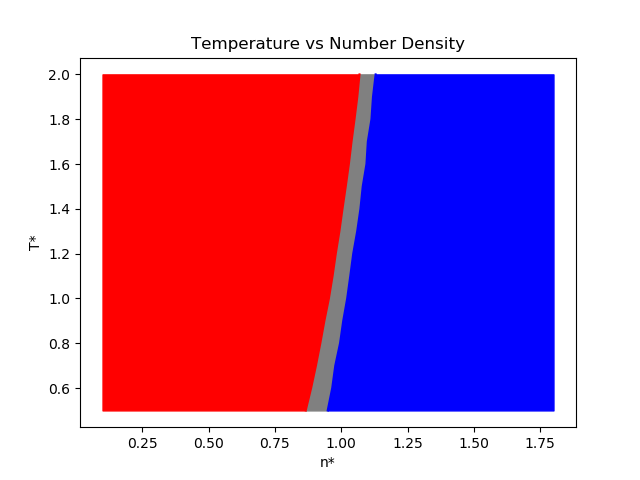
\includegraphics[width=\columnwidth]{figs/Phase_Diagram_of_T_vs_n}
\caption{Phase Diagram of the reduced termperature verses the reduced density. Green lines indicate the region of coexistence from Monte-Carlo simulations.}
\label{fig:Phase_Diagram_of_T_vs_n}
\end{figure}

\begin{figure}
 \begin{center}
  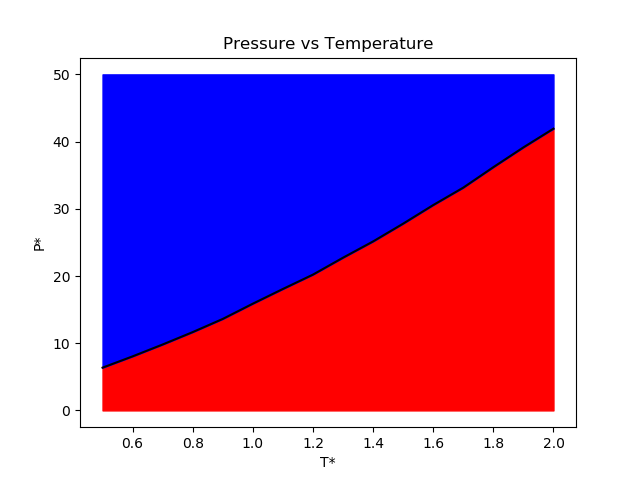
\includegraphics[width=\columnwidth]{figs/Phase_Diagram_of_P_vs_T}
 \end{center}
\caption{Phase Diagram of the reduced pressure verses the reduced temperature. The green line marks the boundary from Monte-Carlo simulations.}
\label{fig:Phase_Diagram_P_vs_T}
\end{figure}

\begin{figure}
 \begin{center}
  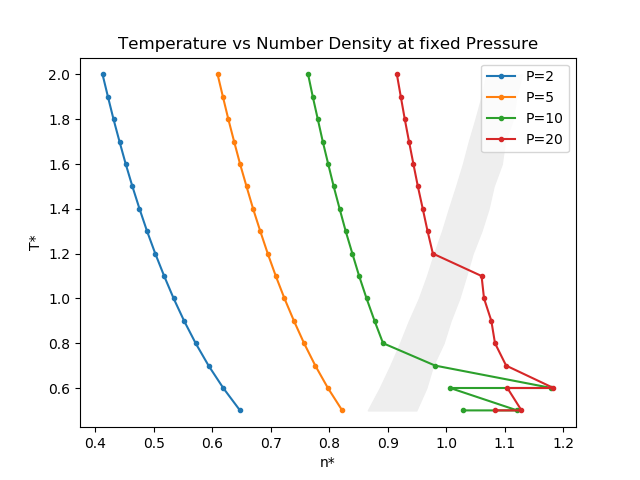
\includegraphics[width=\columnwidth]{figs/T-vs-n_at_fixed_P}
 \end{center}
\caption{Phase Diagram of the reduced temperature verses the reduced density. The grey region indicates coexistence.}
\label{fig:T-vs-n_at_fixed_P}
\end{figure}

\begin{figure}
 \begin{center}
  \includegraphics[width=\columnwidth]{figs/p-vs-T_at_fixed_n}
 \end{center}
\caption{Phase Diagram of the reduced pressure verses the reduced temperature. The lines bending downward indicate freezing.}
\label{fig:p-vs-T_at_fixed_density}
\end{figure}

\begin{figure}
 \begin{center}
  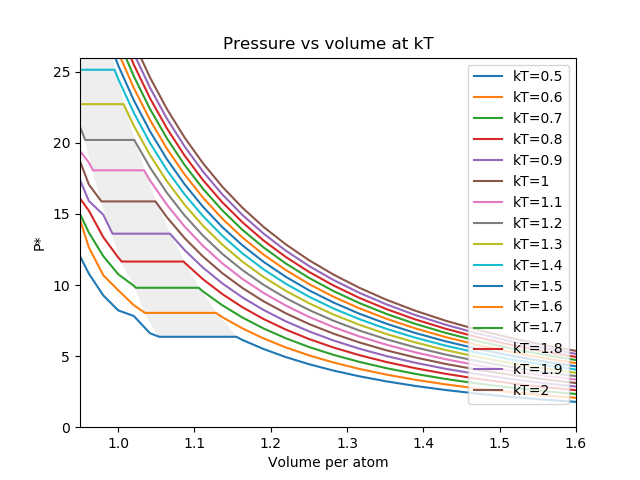
\includegraphics[width=\columnwidth]{figs/p-vs-V_at_fixed_T}
 \end{center}
\caption{Phase Diagram of the reduced pressure verses the reduced volume. The grey region indicates coexistence.}
\label{fig:p-vs-V_at_fixed_T}
\end{figure}

\begin{figure}
 \begin{center}
  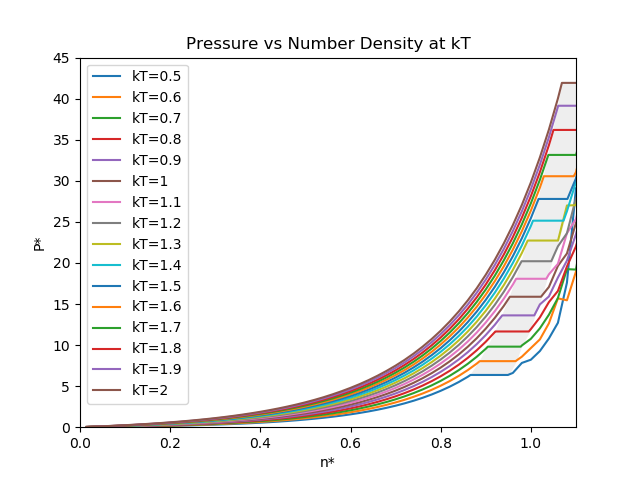
\includegraphics[width=\columnwidth]{figs/p-vs-n_at_fixed_T}
 \end{center}
\caption{Phase Diagram of the reduced pressure verses the reduced density. The grey region indicates coexistence.}
\label{fig:p-vs-n_at_fixed_T}
\end{figure}

\[{}\]
\[{}\]
\[{}\]



\section{Conclusion}

The theory presented in this paper is as good as a Barker-Henderson
hard sphere fluid for a range of densities and temperatures. The
advantage of our theory is that we can use it \emph{as is} rather than
needing to accommodate for discontinuities and delta functions of hard
sphere fluids.

\[{}\]
\[{}\]
\[{}\]
\[{}\]
\[{}\]
\[{}\]
\[{}\]
\[{}\]
\[{}\]
\[{}\]
\[{}\]
\[{}\]
\[{}\]
\[{}\]
\[{}\]
\[{}\]
\[{}\]
\[{}\]
\[{}\]
\[{}\]
\[{}\]
\[{}\]
\[{}\]
\[{}\]
\[{}\]
\[{}\]
\[{}\]
\[{}\]
\[{}\]
\[{}\]
\[{}\]
\[{}\]
\[{}\]
\[{}\]
\[{}\]
\[{}\]
\[{}\]
\[{}\]
\[{}\]
\[{}\]
\[{}\]
\[{}\]
\[{}\]
\[{}\]
\[{}\]
\[{}\]
\[{}\]
\[{}\]

\bibliography{paper}% Produces the bibliography via BibTeX.
 
\begin{widetext}
\[{}\]
%\[{}\]


Appendix
\begin{enumerate}
\item A. Fourier Transfrom of Weight Function $w_0(r)$  
\item B. Foureir Transform of Tensor Weight $\overleftrightarrow{w}_{m2}(r)$
\item C. show trasform of tensor weight $\overleftrightarrow{w}_{m2}(r)$ goes to zero as k goes to 0
\item D. The tensor weight components in the coordinate system (x,y,z) 
\item E. Integrals used to compute tensor weights
\item F. Deriviation of Tensor Density $n_{m2ij}(\vec{r})$ - Work out how tensor weight in Fourier space relates to the tensor density.
\item G. Deriviation of $\Phi_3$ 
\end{enumerate}

%\section{fourier}

\[{}\]
%\tiny
\subsection{Fourier Transform of Weight Function $w_0(r)$}
%\textbf{Weight Function $w_0(r)$:}
\begin{equation}{w_0(r)=\frac{w_2(r)}{4{\pi}r^2}}\end{equation}
where
\begin{equation}{w_2(r)=\frac{\sqrt{2}}{\Xi\sqrt{\pi}}e^{-\left(\frac{r-\frac{\alpha}{2}}{\frac{\Xi}{\sqrt{2}}}\right)^2}}\end{equation}
set 
\begin{equation}{a=\frac{\Xi}{\sqrt{2}}}\end{equation}
\begin{equation}{w_0(r)=\frac{1}{4{\pi}\sqrt{\pi}a}\left(\frac{1}{r^2}\right)e^{-\left(\frac{r-\frac{\alpha}{2}}{a}\right)^2}}\end{equation}
%\[{}\]
\begin{equation}{\widetilde{w}_0(\vec{k})=\int_{0}^{\infty}\int_{-1}^{1}\int_{0}^{2\pi}w_0(r)e^{-i\vec{k}\cdot{\vec{r}}}r^2d{r}d{\cos\theta}d{\phi}}\end{equation}
\begin{equation}{\widetilde{w}_0(k)=\int_{0}^{\infty}\int_{-1}^{1}\int_{0}^{2\pi}w_0(r)e^{-ikr\cos\theta}r^2d{r}d{\cos\theta}d{\phi}}\end{equation}
\[{}\]
Calculate $\widetilde{w}_0(k)$ 
\begin{equation}{\widetilde{w}_0(k)=\frac{1}{4{\pi}\sqrt{\pi}a}\int_{0}^{\infty}\left(\frac{1}{r^2}\right)e^{-\left(\frac{r-\frac{\alpha}{2}}{a}\right)^2}\left[\int_{-1}^{1}e^{-ikr\cos\theta}r^2d{\cos\theta}\left(\int_{0}^{2\pi}d{\phi}\right)\right]d{r}}\end{equation}
\[{}\]
\begin{equation}{\widetilde{w}_0(k)=\frac{2\pi}{4{\pi}\sqrt{\pi}a}\int_{0}^{\infty}e^{-\left(\frac{r-\frac{\alpha}{2}}{a}\right)^2}\left(\int_{-1}^{1}e^{-ikr\cos\theta}d{\cos\theta}\right)d{r}}\end{equation}
\[{}\]
Set the lower limit to -infinity since the integrand is nearly zero by the time r is zero. 
\begin{displaymath}{\widetilde{w}_0(k)=\frac{1}{\sqrt{\pi}ka}\int_{-\infty}^{\infty}e^{-\left(\frac{r-\frac{\alpha}{2}}{a}\right)^2}\frac{\sin(kr)}{r}d{r}}\end{displaymath}
\[{}\]
\begin{equation}{\widetilde{w}_0(k)=\frac{\sqrt{\pi}}{2ka}e^{-\left(\frac{\alpha}{2a}\right)^2}\left[\operatorname{erf}\left(\frac{ka}{2}+i\frac{\alpha}{2a}\right)+\operatorname{erf}\left(\frac{ka}{2}-i\frac{\alpha}{2a}\right)\right]}\end{equation}
\[{}\] %\color{red}
Putting in $a=\frac{\Xi}{\sqrt{2}}$ the final equation for $\widetilde{w}_0(k)$ becomes
\begin{equation}{\widetilde{w}_0(k)=\frac{\sqrt{\pi}}{\sqrt{2}k\Xi}e^{-\left(\frac{\alpha^2}{2\Xi^2}\right)}\left[\operatorname{erf}\left(\frac{k\Xi}{2*\sqrt{2}}+i\frac{\alpha}{\sqrt{2}\Xi}\right)+\operatorname{erf}\left(\frac{k\Xi}{2*\sqrt{2}}-i\frac{\alpha}{\sqrt{2}\Xi}\right)\right]}\end{equation}
\color{black}
\[{}\]

\subsection{Fourier Transform of Weight Function $w_1(r)$}
%\begin{equation}{w_1(r)= }\end{equation}
\begin{equation}
    w_1(k)=\frac{1}{k}e^{-\frac{k^2\Xi^2}{8}}\sin\left(\frac{k\alpha}{2}\right)
\end{equation}

\subsection{Fourier Transform of Weight Function $w_2(r)$}
%\begin{equation}{w_2(r)= }\end{equation}
\begin{equation}{w_2(k)=\frac{2\pi}{k}e^{-\frac{k^2\Xi^2}{8}}\left[\frac{k\Xi^2}{2}\cos\left(\frac{k\alpha}{2}\right)+{\alpha}\sin\left(\frac{k\alpha}{2}\right)\right]}\end{equation}

\subsection{Fourier Transform of Weight Function $w_3(r)$}
\begin{equation}
  w_3(r)=
\end{equation}
\begin{equation}
    w_3(k)=\frac{4\pi}{k^3}
    e^{-\frac{k^2\Xi^2}{8}}
    \left[\left(1+\frac{k^2\Xi^2}{4}\right)\sin\left(\frac{k\alpha}{2}\right)
      -\frac{k\alpha}{2}\cos\left(\frac{k\alpha}{2}\right)\right]
\end{equation}

\subsection{Fourier Transform of Tensor weight ${w}_{m2}(r)$} %$\overleftrightarrow{w}_{m2}(r)$
%\textbf{Tensor Weight $\overleftrightarrow{w}_{m2}(r)$:}
\begin{equation}{\overleftrightarrow{w}_{m2}(\vec{r})=w_2(r)\left(\frac{\vec{r}\vec{r}}{r^2}-\frac{I}{3}\right)}\end{equation}
where
\begin{equation}{w_2(r)=\frac{\sqrt{2}}{\Xi\sqrt{\pi}}e^{-\left(\frac{r-\frac{\alpha}{2}}{\frac{\Xi}{\sqrt{2}}}\right)^2}}\end{equation}
Form the outer product
\begin{equation}{\vec{r}\vec{r}=\left(\begin{array}{c} r_x \\ r_y \\ r_z \end{array} \right) \left(\begin{array}{rrr} r_x & r_y & r_z \end{array} \right)=\left(\begin{array}{ccc} {r^2}_x & r_xr_y & r_xr_z \\ r_yr_x & {r_y}^2 & r_yr_z \\ r_zr_x & r_zr_y & {r_z}^2 \end{array}\right)}\end{equation}
and identity matrix
\begin{equation}{I=\left(\begin{array}{ccc} 1 & 0 & 0 \\ 0 & 1 & 0 \\ 0 & 0 & 1 \end{array}\right)}\end{equation}
The tensor weight matrix elements are then given by
\begin{equation}{w_{m2_{ij}}(\vec{r})=\frac{1}{a\sqrt{\pi}}e^{-\left(\frac{r-\frac{\alpha}{2}}{a}\right)^2}\left(\frac{r_ir_j}{r^2}-\frac{\delta_{ij}}{3}\right)}\end{equation}
with 
\begin{equation}{a=\frac{\Xi}{\sqrt{2}}}\end{equation}
The fourier transform of the tensor weight matrix elements are given by
\begin{equation}{\widetilde{w}_{m2_{ij}}(\vec{k})=\int_{allspace}{w_{{m2}_{ij}}}(\vec{r})e^{-i\vec{k}\cdot\vec{r}}d{\vec{r}}}\end{equation}
%\mbox{~%\scriptsize\textbullet~}
Since the integration is over all space, the integral can be simplified by setting 
\begin{equation}{\vec{k}=k\hat{z}=k\cos\theta\hat{z}}\end{equation}
Instead of constraining vector $\vec{k}$ to be in the z direction, however, a rotated coordinate system $(x',y',z')$ is used which is rotated from the (x,y,z) coordinate system in such a way that $z'$ points in the direction of vector $\vec{k}$. After solving for the elements of the transformed weight function in coordinate system $(x',y',z')$, they will be expressed again in terms of vector $\vec{k}$ as it appears in coordinate system (x,y,z) to get the elements of the transformed weight function in coordinate system (x,y,z).

%The weight components of interest are those corresponding to the component of vector $\vec{r}$ parallel to vector $\vec{k}$ which will be called $r_{z'}$, and to the two components of $\vec{r}$ perpendicular to vector $\vec{k}$ (and to each other) which will be called $r_{x'}$ and $r_{y'}$. 
\begin{equation}{\widetilde{w}_{m2_{ij}}(k)=\frac{1}{a\sqrt{\pi}}\int_{0}^{\infty}\int_{-1}^{1}\int_{0}^{2\pi}e^{-\left(\frac{r-\frac{\alpha}{2}}{a}\right)^2}\left(\frac{r_ir_j}{r^2}-\frac{\delta_{ij}}{3}\right)e^{-ikr\cos\theta'}r^2d{r}d{\cos\theta'}d{\phi'}}\end{equation}
%\begin{displaymath}{r_x=r\sin(\theta)\cos(\phi) ~~~~~ r_y=r\sin(\theta)\sin(\phi)~~~~~ r_z=r\cos(\theta)}\end{displaymath}
where $r=r'$ and
\begin{displaymath}{r_{x'}=r\sin\theta\cos\phi}\end{displaymath}
\begin{displaymath}{r_{y'}=r\sin\theta\sin\phi}\end{displaymath}
\begin{displaymath}{r_{z'}=r\cos\theta}\end{displaymath} 
with
\begin{displaymath}{\delta_{ij}=\left\{ \begin{array}{rc} 1 & i = j \\ 0  & i\neq j \end{array}\right.}\end{displaymath}
\[{}\]

%\[{}\]
%\[{}\]
Calculate $\widetilde{w}_{{m2}_{x'y'}}(k)$ 
%where \begin{displaymath}{r_x=r\sin(\theta)\cos(\phi)}\end{displaymath}
%\begin{displaymath}{r_y=r\sin(\theta)\sin(\phi)}\end{displaymath}
\begin{equation}{\widetilde{w}_{{m2}_{x'y'}}(k)=\frac{1}{a\sqrt{\pi}}\int_{0}^{\infty}\int_{-1}^{1}\int_{0}^{2\pi}e^{-\left(\frac{r-\frac{\alpha}{2}}{a}\right)^2}\left(\frac{(r_{x'})(r_{y'})}{r^2}-\frac{\delta_{x'y'}}{3}\right)e^{-ikr\cos\theta'}r^2d{r}d{\cos\theta'}d{\phi'}}\end{equation}
\begin{equation}{\widetilde{w}_{{m2}_{x'y'}}(k)=\frac{1}{a\sqrt{\pi}}\int_{0}^{\infty}\int_{-1}^{1}e^{-\left(\frac{r-\frac{\alpha}{2}}{a}\right)^2}r^2e^{-ikr\cos\theta'}\sin^2\theta'\underbrace{\left(\int_{0}^{2\pi}\cos\phi'\sin{\phi'}~d{\phi'}\right)}d{r}d{\cos\theta'}=0}\end{equation}
$~~~~~~~~~~~~~~~~~~~~~~~~~~~~~~~~~~~~~~~~~~~~~~~~~~~~~~~~~~~~~~~~~~~~~~~~~~~~~~~~~~~~~~~~~~~~~~~~~~~~~~~~0$

Calculate $\widetilde{w}_{{m2}_{x'z'}}(k)$ 
\begin{equation}{\widetilde{w}_{{m2}_{x'z'}}(k)=\frac{1}{a\sqrt{\pi}}\int_{0}^{\infty}\int_{-1}^{1}\int_{0}^{2\pi}e^{-\left(\frac{r-\frac{\alpha}{2}}{a}\right)^2}\left(\frac{(r_{x'})(r_{z'})}{r^2}-\frac{\delta_{x'z'}}{3}\right)e^{-ikr\cos\theta'}r^2d{r}d{\cos\theta'}d{\phi'}}\end{equation}
\begin{equation}{\widetilde{w}_{{m2}_{x'z'}}(k)=\frac{1}{a\sqrt{\pi}}\int_{0}^{\infty}\int_{-1}^{1}e^{-\left(\frac{r-\frac{\alpha}{2}}{a}\right)^2}r^2e^{-ikr\cos\theta'}\sin\theta'\cos\theta'\underbrace{\left(\int_{0}^{2\pi}\cos\phi'~d{\phi'}\right)}d{r}d{\cos\theta'}=0}\end{equation}
$~~~~~~~~~~~~~~~~~~~~~~~~~~~~~~~~~~~~~~~~~~~~~~~~~~~~~~~~~~~~~~~~~~~~~~~~~~~~~~~~~~~~~~~~~~~~~~~~~~~~~~~~~~~0$
\[{}\]
Calculate $\widetilde{w}_{{m2}_{y'z'}}(k)$ 
\begin{equation}{\widetilde{w}_{{m2}_{y'z'}}(\vec{k})=\frac{1}{a\sqrt{\pi}}\int_{0}^{\infty}\int_{-1}^{1}\int_{0}^{2\pi}e^{-\left(\frac{r-\frac{\alpha}{2}}{a}\right)^2}\left(\frac{(r_{y'})(r_{z'})}{r^2}-\frac{\delta_{yz}}{3}\right)e^{-ikr\cos\theta'}r^2d{r}d{\cos\theta'}d{\phi'}}\end{equation}
\begin{equation}{\widetilde{w}_{{m2}_{y'z'}}(\vec{k})=\frac{1}{a\sqrt{\pi}}\int_{0}^{\infty}\int_{-1}^{1}e^{-\left(\frac{r-\frac{\alpha}{2}}{a}\right)^2}r^2e^{-ikr\cos\theta'}\sin\theta'\cos\theta'\underbrace{\left(\int_{0}^{2\pi}\sin\phi'~d{\phi'}\right)}d{r}d{\cos\theta'}=0}\end{equation}
$~~~~~~~~~~~~~~~~~~~~~~~~~~~~~~~~~~~~~~~~~~~~~~~~~~~~~~~~~~~~~~~~~~~~~~~~~~~~~~~~~~~~~~~~~~~~~~~~~~~~~~~~~~~0$
\[{}\]
Calculate $\widetilde{w}_{{m2}_{x'x'}}(k)$ 
\begin{equation}{\widetilde{w}_{{m2}_{x'x'}}(k)=\frac{1}{a\sqrt{\pi}}\int_{0}^{\infty}\int_{-1}^{1}\int_{0}^{2\pi}e^{-\left(\frac{r-\frac{\alpha}{2}}{a}\right)^2}\left(\frac{(r_{x'})(r_{x'})}{r^2}-\frac{\delta_{x'x'}}{3}\right)e^{-ikr\cos\theta'}r^2d{r}d{\cos\theta'}d{\phi'}}\end{equation}
\begin{equation}{\widetilde{w}_{{m2}_{x'x'}}(k)=\frac{1}{a\sqrt{\pi}}\int_{0}^{\infty}\int_{-1}^{1}\int_{0}^{2\pi}e^{-\left(\frac{r-\frac{\alpha}{2}}{a}\right)^2}\left(\sin^2\theta'\cos^2\phi'-\frac{1}{3}\right)e^{-ikr\cos\theta'}r^2d{r}d{\cos\theta'}d{\phi'}}\end{equation}
\[{}\]
%\[{}\]
%\begin{displaymath}{\widetilde{w}_{{m2}_{xx}}(\vec{k})=\frac{1}{a\sqrt{\pi}}\int_{0}^{\infty}e^{\left(\frac{r-\frac{\alpha}{2}}{a}\right)^2}r^2\left[\int_{-1}^{1}\sin^2(\theta)e^{-ikr\cos(\theta)}\left(\int_{0}^{2\pi}\cos^2(\phi)d{\phi}\right)d{\cos(\theta)}\right]d{r}}\end{displaymath} 
\begin{displaymath}{\widetilde{w}_{{m2}_{x'x'}}(k)=\frac{1}{a\sqrt{\pi}}\int_{0}^{\infty}e^{-\left(\frac{r-\frac{\alpha}{2}}{a}\right)^2}r^2\left[\int_{-1}^{1}\left(1-\cos^2\theta'\right)e^{-ikr\cos\theta'}\left(\int_{0}^{2\pi}\cos^2\phi'~d{\phi'}\right)d{\cos\theta'}\right]d{r}}\end{displaymath} 
\begin{equation}{-\frac{1}{3a\sqrt{\pi}}\int_{0}^{\infty}e^{-\left(\frac{r-\frac{\alpha}{2}}{a}\right)^2}r^2\left[\int_{-1}^{1}e^{-ikr\cos\theta'}\left(\int_{0}^{2\pi}d{\phi'}\right)d{\cos\theta'}\right]d{r}}\end{equation}
\[{}\]
\color{blue}
\begin{displaymath}{\widetilde{w}_{{m2}_{x'x'}}(k)=-\frac{\sqrt{\pi}}{a}\int_{0}^{\infty}e^{-\left(\frac{r-\frac{\alpha}{2}}{a}\right)^2}r^2\left[\int_{-1}^{1}\cos^2\theta'~e^{-ikr\cos\theta'}~d{\cos\theta'}\right]d{r}}\end{displaymath} 
\begin{equation}\label{compare_equation}{+\frac{\sqrt{\pi}}{3a}\int_{0}^{\infty}e^{-\left(\frac{r-\frac{\alpha}{2}}{a}\right)^2}r^2\left[\int_{-1}^{1}e^{-ikr\cos\theta'}~d{\cos\theta'}\right]d{r}}\end{equation}
\color{black}
\[{}\]
\begin{displaymath}{\widetilde{w}_{{m2}_{x'x'}}(k)=-\frac{\sqrt{\pi}}{a}\int_{0}^{\infty}e^{-\left(\frac{r-\frac{\alpha}{2}}{a}\right)^2}r^2\left(\frac{2\sin(kr)}{kr}+\frac{4\cos(kr)}{k^2r^2}-\frac{4\sin(kr)}{k^3r^3}\right)d{r}}\end{displaymath} 
\begin{equation}{+\frac{\sqrt{\pi}}{3a}\int_{0}^{\infty}e^{-\left(\frac{r-\frac{\alpha}{2}}{a}\right)^2}r^2\left(\frac{2\sin(kr)}{kr}\right)d{r}}\end{equation}
%\[{}\]
Set the lower limit to -infinity since the integrand is nearly zero by the time r is zero. 
\begin{displaymath}{\widetilde{w}_{{m2}_{x'x'}}(k)=-\frac{4\sqrt{\pi}}{3ka}\left(\int_{-\infty}^{\infty}e^{-\left(\frac{r-\frac{\alpha}{2}}{a}\right)^2}r\sin(kr)d{r}\right)}\end{displaymath} 
\begin{displaymath}{-\frac{4\sqrt{\pi}}{k^2a}\left(\int_{-\infty}^{\infty}e^{-\left(\frac{r-\frac{\alpha}{2}}{a}\right)^2}\cos(kr)d{r}\right)}\end{displaymath} 
\begin{equation}{+\frac{4\sqrt{\pi}}{k^3a}\left(\int_{-\infty}^{\infty}e^{-\left(\frac{r-\frac{\alpha}{2}}{a}\right)^2}\frac{\sin(kr)}{r}d{r}\right)}\end{equation} 
\[{}\]
\begin{displaymath}{\widetilde{w}_{{m2}_{x'x'}}(k)=\frac{-4\sqrt{\pi}}{3ka}\left(\frac{ka^3}{2}\sqrt{\pi}e^{-\left(\frac{ka}{2}\right)^2}\cos(\frac{k\alpha}{2})+\frac{a\alpha}{2}\sqrt{\pi}e^{-\left(\frac{ka}{2}\right)^2}\sin(\frac{k\alpha}{2})\right)}\end{displaymath} 
\begin{displaymath}{-\frac{4\sqrt{\pi}}{k^2a}\left(a\sqrt{\pi}e^{-\left(\frac{ka}{2}\right)^2}\cos(\frac{k\alpha}{2})\right)}\end{displaymath} 
\begin{equation}{+\frac{4\sqrt{\pi}}{k^3a}\left(\frac{\pi}{2}e^{-\left(\frac{\alpha}{2a}\right)^2}\left[\operatorname{erf}\left(\frac{ka}{2}+i\frac{\alpha}{2a}\right)+\operatorname{erf}\left(\frac{ka}{2}-i\frac{\alpha}{2a}\right)\right]\right)}\end{equation} 
\[{}\]
\begin{displaymath}{\widetilde{w}_{{m2}_{x'x'}}(k)=\left(\frac{-2\pi{a}^2}{3}-\frac{4\pi}{k^2}\right)e^{-\left(\frac{ka}{2}\right)^2}   \cos(\frac{k\alpha}{2})-\frac{2\pi\alpha}{3k}e^{-\left(\frac{ka}{2}\right)^2}\sin(\frac{k\alpha}{2})}\end{displaymath} 
\begin{equation}{+\frac{2\pi\sqrt{\pi}}{k^3a}e^{-\left(\frac{\alpha}{2a}\right)^2}\left[\operatorname{erf}\left(\frac{ka}{2}+i\frac{\alpha}{2a}\right)+\operatorname{erf}\left(\frac{ka}{2}-i\frac{\alpha}{2a}\right)\right]}\end{equation} 
\[{}\] 
Putting in $a=\frac{\Xi}{\sqrt{2}}$ the final equation for $\widetilde{w}_{{m2}_{xx}}(k)$ becomes
\color{green}
\begin{displaymath}{\widetilde{w}_{{m2}_{x'x'}}(k)=\left(\frac{-\pi\Xi^2}{3}-\frac{4\pi}{k^2}\right)e^{-\left(\frac{k^2\Xi^2}{8}\right)}\cos(\frac{k\alpha}{2})-\frac{2\pi\alpha}{3k}e^{-\left(\frac{k^2\Xi^2}{8}\right)}\sin(\frac{k\alpha}{2})}\end{displaymath} 
\begin{equation}{+\frac{2\pi\sqrt{2\pi}}{k^3\Xi}e^{-\left(\frac{\alpha^2}{2\Xi^2}\right)}\left[\operatorname{erf}\left(\frac{k\Xi}{2*\sqrt{2}}+i\frac{\alpha}{\sqrt{2}\Xi}\right)+\operatorname{erf}\left(\frac{k\Xi}{2*\sqrt{2}}-i\frac{\alpha}{\sqrt{2}\Xi}\right)\right]}\end{equation} 
\color{black}
\[{}\]
 
Calculate $\widetilde{w}_{{m2}_{y'y'}}(k)$ 
\begin{equation}{\widetilde{w}_{{m2}_{y'y'}}(k)=\frac{1}{a\sqrt{\pi}}\int_{0}^{\infty}\int_{-1}^{1}\int_{0}^{2\pi}e^{-\left(\frac{r-\frac{\alpha}{2}}{a}\right)^2}\left(\frac{(r_{y'})(r_{y'})}{r^2}-\frac{\delta_{y'y'}}{3}\right)e^{-ikr\cos\theta'}r^2d{r}d{\cos\theta'}d{\phi'}}\end{equation}
\begin{equation}{\widetilde{w}_{{m2}_{y'y'}}(k)=\frac{1}{a\sqrt{\pi}}\int_{0}^{\infty}\int_{-1}^{1}\int_{0}^{2\pi}e^{-\left(\frac{r-\frac{\alpha}{2}}{a}\right)^2}\left(\sin^2\theta'\sin^2\phi'-\frac{1}{3}\right)e^{-ikr\cos\theta'}r^2d{r}d{\cos\theta'}d{\phi'}}\end{equation}
\[{}\]
\begin{displaymath}{\widetilde{w}_{{m2}_{y'y'}}(k)=\frac{1}{a\sqrt{\pi}}\int_{0}^{\infty}e^{-\left(\frac{r-\frac{\alpha}{2}}{a}\right)^2}r^2\left[\int_{-1}^{1}\left(1-\cos^2\theta\right)e^{-ikr\cos\theta'}\left(\int_{0}^{2\pi}\sin^2\phi~d{\phi}\right)d{\cos\theta}\right]d{r}}\end{displaymath} 
\begin{equation}{-\frac{1}{3a\sqrt{\pi}}\int_{0}^{\infty}e^{-\left(\frac{r-\frac{\alpha}{2}}{a}\right)^2}r^2\left[\int_{-1}^{1}e^{-ikr\cos\theta'}\left(\int_{0}^{2\pi}d{\phi'}\right)d{\cos\theta'}\right]d{r}}\end{equation}

\color{blue}
\begin{displaymath}{\widetilde{w}_{{m2}_{y'y'}}(k)=-\frac{\sqrt{\pi}}{a}\int_{0}^{\infty}e^{-\left(\frac{r-\frac{\alpha}{2}}{a}\right)^2}r^2\left[\int_{-1}^{1}\cos^2\theta~e^{-ikr\cos\theta'}~d{\cos\theta'}\right]d{r}}\end{displaymath} 
\begin{equation}{+\frac{\sqrt{\pi}}{3a}\int_{0}^{\infty}e^{-\left(\frac{r-\frac{\alpha}{2}}{a}\right)^2}r^2\left[\int_{-1}^{1}e^{-ikr\cos\theta'}~d{\cos\theta'}\right]d{r}}\end{equation}
\color{black} 
\[{}\]

%HEREEEE!!!!

This is the same as equation \ref{compare_equation}, and so \begin{equation}{\widetilde{w}_{{m2}_{y'y'}}(k)=\widetilde{w}_{{m2}_{x'x'}}(k)}\end{equation}
Calculate $\widetilde{w}_{{m2}_{z'z'}}(k)$ 
\begin{equation}{\widetilde{w}_{{m2}_{z'z'}}(k)=\frac{1}{a\sqrt{\pi}}\int_{0}^{\infty}\int_{-1}^{1}\int_{0}^{2\pi}e^{\left(\frac{r-\frac{\alpha}{2}}{a}\right)^2}\left(\frac{(r_{y'})(r_{y'})}{r^2}-\frac{\delta_{z'z'}}{3}\right)e^{-ikr\cos\theta'}r^2d{r}d{\cos\theta'}d{\phi'}}\end{equation}
\begin{equation}{\widetilde{w}_{{m2}_{z'z'}}(k)=\frac{1}{a\sqrt{\pi}}\int_{0}^{\infty}\int_{-1}^{1}\int_{0}^{2\pi}e^{\left(\frac{r-\frac{\alpha}{2}}{a}\right)^2}\left(\cos^2\theta'-\frac{1}{3}\right)e^{-ikr\cos\theta'}r^2d{r}d{\cos\theta'}d{\phi'}}\end{equation}
\[{}\]
\begin{displaymath}{\widetilde{w}_{{m2}_{z'z'}}(k)=\frac{1}{a\sqrt{\pi}}\int_{0}^{\infty}e^{-\left(\frac{r-\frac{\alpha}{2}}{a}\right)^2}r^2\left[\int_{-1}^{1}\cos^2\theta'~e^{-ikr\cos\theta'}\left(\int_{0}^{2\pi}d{\phi'}\right)d{\cos\theta'}\right]d{r}}\end{displaymath} 
\begin{equation}{-\frac{1}{3a\sqrt{\pi}}\int_{0}^{\infty}e^{-\left(\frac{r-\frac{\alpha}{2}}{a}\right)^2}r^2\left[\int_{-1}^{1}e^{-ikr\cos\theta'}\left(\int_{0}^{2\pi}d{\phi'}\right)d{\cos\theta'}\right]d{r}}\end{equation}

\color{blue}
\begin{displaymath}{\widetilde{w}_{{m2}_{z'z'}}(k)=2\frac{\sqrt{\pi}}{a}\int_{0}^{\infty}e^{-\left(\frac{r-\frac{\alpha}{2}}{a}\right)^2}r^2\left[\int_{-1}^{1}\cos^2\theta'~e^{-ikr\cos\theta'}d{\cos\theta'}\right]d{r}}\end{displaymath} 
\begin{equation}{-2\frac{\sqrt{\pi}}{3a}\int_{0}^{\infty}e^{-\left(\frac{r-\frac{\alpha}{2}}{a}\right)^2}r^2\left[\int_{-1}^{1}e^{-ikr\cos\theta'}d{\cos\theta'}\right]d{r}}\end{equation}
\color{black} 


%HEREEEE!!!!


This is the same as -2 times equation \ref{compare_equation}, and so \begin{equation}{\widetilde{w}_{{m2}_{z'z'}}(k)=-2\widetilde{w}_{{m2}_{x'x'}}(k)}\end{equation}
\[{}\]
%GOOD TO HERE
\subsection{Transform of tensor weight ${w}_{m2}(r)$ goes to zero as k goes to zero}
\begin{displaymath}{\widetilde{w}_{{m2}_{x'x'}}(k)=\left(\frac{-\pi\Xi^2}{3}-\frac{4\pi}{k^2}\right)e^{-\left(\frac{k^2\Xi^2}{8}\right)}\cos(\frac{k\alpha}{2})-\frac{2\pi\alpha}{3k}e^{-\left(\frac{k^2\Xi^2}{8}\right)}\sin(\frac{k\alpha}{2})}\end{displaymath} 
\begin{equation}{+\frac{2\pi\sqrt{2\pi}}{k^3\Xi}e^{-\left(\frac{\alpha^2}{2\Xi^2}\right)}\left[\operatorname{erf}\left(\frac{k\Xi}{2*\sqrt{2}}+i\frac{\alpha}{\sqrt{2}\Xi}\right)+\operatorname{erf}\left(\frac{k\Xi}{2*\sqrt{2}}-i\frac{\alpha}{\sqrt{2}\Xi}\right)\right]}\end{equation}
Term 1: 
\color{green}
\begin{equation}{\left(\frac{-\pi\Xi^2}{3}-\frac{4\pi}{k^2}\right)e^{-\left(\frac{k^2\Xi^2}{8}\right)}\cos(\frac{k\alpha}{2})}\end{equation}
\begin{displaymath}{\approx\left(-\frac{\pi\Xi^2}{3}-\frac{4\pi}{k^2}\right)\left(1-\frac{k^2\Xi^2}{8}\right)\left(1-\left(\frac{1}{2}\right)\frac{k^2\alpha^2}{4}\right)}\end{displaymath} 
\begin{displaymath}{\approx-\frac{4\pi}{k^2}+\frac{\pi\alpha^2}{2}+\frac{\pi\Xi^2}{6}}\end{displaymath} 
\color{black}
Term 2:
\color{blue}
\begin{equation}{-\frac{2\pi\alpha}{3k}e^{-\left(\frac{k^2\Xi^2}{8}\right)}\sin(\frac{k\alpha}{2})}\end{equation} 
\begin{displaymath}{\approx\left(-\frac{2\pi\alpha}{3k}\right)\left(1-\frac{k^2\Xi^2}{8}\right)\left(\frac{k\alpha}{2}\right)}\end{displaymath} 
\begin{displaymath}{\approx}-\frac{\pi\alpha^2}{3}\end{displaymath}
\color{black} 
Term 3:
\color{red}
\begin{equation}{\frac{2\pi\sqrt{2\pi}}{k^3\Xi}e^{-\left(\frac{\alpha^2}{2\Xi^2}\right)}\left[\operatorname{erf}\left(\frac{k\Xi}{2*\sqrt{2}}+i\frac{\alpha}{\sqrt{2}\Xi}\right)+\operatorname{erf}\left(\frac{k\Xi}{2*\sqrt{2}}-i\frac{\alpha}{\sqrt{2}\Xi}\right)\right]}\end{equation}
\begin{displaymath}{\approx\frac{\left(2\pi\right)^\frac{2}{3}}{\Xi{k}^3}e^{-\left(\frac{\alpha^2}{2\Xi^2}\right)}\left[2\operatorname{Re}\left(\operatorname{erf}\left(\frac{k\Xi}{2\sqrt{2}}+i\frac{\alpha}{\sqrt{2}\Xi}\right)\right)\right]}\end{displaymath} 
\begin{displaymath}{\approx\frac{\left(2\pi\right)^\frac{2}{3}}{\Xi{k}^3}e^{-\left(\frac{\alpha^2}{2\Xi^2}\right)}\left[2e^{\left(\frac{\alpha^2}{2\Xi^2}\right)}\frac{2}{\sqrt{\pi}}   \left(\frac{k\Xi}{2\sqrt{2}}   -\frac{2\left(\frac{\alpha^2}{2\Xi^2}\right)+1}{3}\left(\frac{k\Xi}{2\sqrt{2}}\right)^3\right)\right]}\end{displaymath}
\begin{displaymath}{\approx\frac{4\pi}{k^2}-\frac{\pi}{6}\left(\alpha^2-\Xi^2\right)}\end{displaymath}  
\color{black}
Adding the three terms gives:
\begin{displaymath}{\approx-\frac{4\pi}{k^2}+\frac{\pi\alpha^2}{2}+\frac{\pi\Xi^2}{6}-\frac{\pi\alpha^2}{3}+\frac{4\pi}{k^2}-\frac{\pi\alpha^2}{6}-\frac{\pi\Xi^2}{6}}\end{displaymath} 
\begin{displaymath}{\approx0}\end{displaymath} 
\[{}\]


\subsection{The tensor weight components in the coordinate system (x,y,z)}
The tensor weight components in the coordinate system $(x',y',z')$ are:
\begin{equation}{\widetilde{w'}_{m2}=\left(\begin{array}{ccc} \widetilde{w}_{{m2}_{x'x'}} & 0 & 0 \\ 0 & \widetilde{w}_{{m2}_{y'y'}} & 0 \\ 0 & 0 & \widetilde{w}_{{m2}_{z'z'}} \end{array}\right)'}\end{equation}
\begin{displaymath}{=\widetilde{w}_{{m2}_{x'x'}}\hat{x'}\hat{x'}+\widetilde{w}_{{m2}_{y'y'}}\hat{y'}\hat{y'}+\widetilde{w}_{{m2}_{z'z'}}\hat{z'}\hat{z'}}\end{displaymath}
where vector had been aligned with the $\hat{z}$ direction so that 
\begin{equation}{\hat{k}=\hat{z'}}\end{equation}
%\newline $k_{x'}= k_{x'_x} \hat{x} + k_{x'_y} \hat{y} + k_{x'_z} \hat{z}$
%\newline $k_{y'}= k_{y'_x} \hat{x} + k_{y'_y} \hat{y} + k_{y'_z} \hat{z}$
%\newline $k_{z'}= k_{z'_x} \hat{x} + k_{z'_y} \hat{y} + k_{z'_z} \hat{z}$
%\newline \begin{displaymath}{\widetilde{w}_{{m2}_{y'y'}}(\vec{k})=\widetilde{w}_{{m2}_{x'x'}}(\vec{k})}\end{displaymath}
Using the relation
%\begin{displaymath}{\hat{k_{x'}}\hat{k_{x'}} + \hat{k_{y'}}\hat{k_{y'}} + \hat{k_{z'}}\hat{k_{z'}} = 1}\end{displaymath} 
\begin{displaymath}{1 = \hat{x'}\hat{x'} + \hat{y'}\hat{y'} + \hat{z'}\hat{z'}}\end{displaymath}
\begin{displaymath}{1 -\hat{z'}\hat{z'} = \hat{x'}\hat{x'} + \hat{y'}\hat{y'}}\end{displaymath}
and the results from earlier
\begin{equation}{\widetilde{w}_{{m2}_{y'y'}}=\widetilde{w}_{{m2}_{x'x'}}}\end{equation}
\begin{equation}{\widetilde{w}_{{m2}_{z'z'}}=-2\widetilde{w}_{{m2}_{x'x'}}}\end{equation}
results in
\begin{displaymath}{\widetilde{w}_{m2}(\vec{k})= (1-3\hat{k}\hat{k})\widetilde{w}_{{m2}_{x'x'}}(\vec{k})}\end{displaymath}
and so 
\begin{displaymath}{\widetilde{w}_{m2_{ij}}(\vec{k})= (\delta{ij}-3k_ik_j)\widetilde{w}_{{m2}_{x'x'}}(\vec{k})}\end{displaymath}
\[{}\]


\[{}\]
\subsection{Integrals used to compute tensor weights}
%\textbf{Integrals used to compute tensor weights:}
\begin{equation}{\int_{-1}^{1}{e^{-ikr\cos{\theta}}d{\cos{\theta}}}=\frac{2\sin(kr)}{kr}}\end{equation} 
\[{}\]
\begin{equation}{\int_{-1}^{1}{e^{-ikr\cos{\theta}}\cos^2(\theta)~d{\cos{\theta}}}=\frac{2\sin(kr)}{kr}+\frac{4\cos(kr)}{k^2r^2}-\frac{4\sin(kr)}{k^3r^3}}\end{equation} 
\[{}\]
\[{}\]
\begin{equation}{\int_{-\infty}^{\infty}{e^{-\left(\frac{r-\frac{\alpha}{2}}{a}\right)^2}\cos(kr)d{r}}}\end{equation}
\begin{displaymath}{=a\int_{-\infty}^{\infty}{e^{-u^2}\left[\cos(kau)\cos(\frac{k\alpha}{2})-\sin(kau)\sin(\frac{k\alpha}{2})\right]d{u}}}\end{displaymath}  
\begin{equation}{=a\sqrt{\pi}e^{-\left(\frac{ka}{2}\right)^2}\cos(\frac{k\alpha}{2})}\end{equation} 
\[{}\]
\begin{equation}{\int_{-\infty}^{\infty}{e^{-\left(\frac{r-\frac{\alpha}{2}}{a}\right)^2}r\sin(kr)d{r}}}\end{equation} 
\begin{displaymath}{=a\int_{-\infty}^{\infty}{e^{-u^2}(au+\frac{\alpha}{2})\sin(k(au+\frac{\alpha}{2}))d{u}}}\end{displaymath} 
\begin{displaymath}{=a^2\cos(\frac{k\alpha}{2})\int_{-\infty}^{\infty}{e^{-u^2}u\sin(kau)d{u} +\frac{a\alpha}{2}\sin(\frac{k\alpha}{2})\int_{-\infty}^{\infty}e^{-u^2}\cos(kau)d{u}}}\end{displaymath} 
\begin{equation}{=\frac{ka^3}{2}\sqrt{\pi}e^{-\left(\frac{ka}{2}\right)^2}\cos(\frac{k\alpha}{2})+\frac{a\alpha}{2}\sqrt{\pi}e^{-\left(\frac{ka}{2}\right)^2}\sin(\frac{k\alpha}{2})}\end{equation} 
%\[{}\]
\[{}\]
\begin{equation}{\int_{-\infty}^{\infty}{e^{-\left(\frac{r-\frac{\alpha}{2}}{a}\right)^2}\frac{\sin(kr)}{r}d{r}}}\end{equation} 
%Noting that \begin{equation}{\frac{\sin(kr)}{r}=\int_{0}^{k}{\cos(kr)d{k}}}\end{equation} 
%this becomes
\begin{displaymath}{=\int_{-\infty}^{\infty}{e^{-\left(\frac{r-\frac{\alpha}{2}}{a}\right)^2}\left(\int_{0}^{k}{\cos(kr)d{k}}\right)d{r}}}\end{displaymath} 
\begin{displaymath}{=\int_{0}^{k}\int_{-\infty}^{\infty}{e^{-\left(\frac{r-\frac{\alpha}{2}}{a}\right)^2}{\cos(kr)d{r}}d{k}}}\end{displaymath} 
\begin{displaymath}{=a\sqrt{\pi}\int_{0}^{k}e^{-\left(\frac{ka}{2}\right)^2}\cos\left(\frac{k\alpha}{2}\right)d{k} }\end{displaymath} 
%\begin{displaymath}{=a\sqrt{\pi}\int_{0}^{k}e^{-\left(\frac{ka}{2}\right)^2}\left(\frac{e^{i\frac{k\alpha}{2}}+e^{-i\frac{k\alpha}{2}}}{2}\right)d{k} }\end{displaymath} 
%\begin{displaymath}{=\frac{a\sqrt{\pi}}{2}\left[\int_{0}^{k}e^{-\left(\frac{ka}{2}\right)^2 + i\frac{k\alpha}{2}}d{k}+\int_{0}^{k}e^{-\left(\frac{ka}{2}\right)^2-i\frac{k\alpha}{2}}d{k}\right]}\end{displaymath} 
\begin{displaymath}{=\frac{a\sqrt{\pi}}{2}\left[\int_{-k}^{k}e^{-\left(\frac{ka}{2}\right)^2 + i\frac{k\alpha}{2}}d{k}\right]}\end{displaymath} 
%\begin{displaymath}{=\frac{a\sqrt{\pi}}{2}e^{-\left(\frac{\alpha}{2a}\right)^2}\left[\int_{-k}^{k}e^{-\left(\frac{ka}{2} + i\frac{\alpha}{2a}\right)^2}d{k}\right]}\end{displaymath} 
\begin{displaymath}{=\sqrt{\pi}e^{-\left(\frac{\alpha}{2a}\right)^2}\int_{-\frac{ka}{2}+i\frac{\alpha}{2a}}^{\frac{ka}{2}+i\frac{\alpha}{2a}}e^{-u^2}d{u}}\end{displaymath} 
\begin{equation}{=\frac{\pi}{2}e^{-\left(\frac{\alpha}{2a}\right)^2}\left[\operatorname{erf}\left(\frac{ka}{2}+i\frac{\alpha}{2a}\right)+\operatorname{erf}\left(\frac{ka}{2}-i\frac{\alpha}{2a}\right)\right]}\end{equation} 
\[{}\]
\[{}\]

\subsection{Deriviation of Tensor Density} 
%Work out how tensor weight in Fourier space relates to the tensor density:
\noindent The tensor density is given by:
\begin{equation}{\overleftrightarrow{n}_{m2}(\vec{r})=\int_{allspace}n(\vec{r'})\overleftrightarrow{w}_{m2}(|\vec{r}-\vec{r'}|)d{\vec{r'}}}\end{equation}
%ERROR below?? Shoud it be:
with tensor elements  
\begin{displaymath}{n_{m2_{ij}}(\vec{r})=\int_{allspace}n(\vec{r'})w_{m2_{ij}}(|\vec{r}-\vec{r'}|)d{r'}}\end{displaymath} 
where
\begin{equation}{w_{m2ij}(\vec r)= \frac1{2\pi}\int d\vec k w_{m2ij}(\vec k)e^{i\vec k\cdot \vec r}}\end{equation} 
Deriviation of tensor density elements $n_{m2ij}(\vec{r})$:
\begin{align}
%    n_{m2ij}(\vec r) &= \int_{allspace} n(\vec r') w_{m2ij}(\vec r- \vec r')d\vec r' \\
%    w_{m2ij}(\vec r) &= \frac1{2\pi}\int d\vec k w_{m2ij}(\vec k)e^{i\vec k\cdot \vec r}\\
    n_{m2ij}(\vec r) &= \int n(\vec r') d\vec r' \frac1{2\pi}\int d\vec k w_{m2ij}(\vec k)e^{i\vec k\cdot (\vec r-\vec r')} \\
    &= \int d\vec r' \left(\frac1{2\pi}\int d\vec k' n(\vec k')e^{i\vec k'\cdot \vec r'}\right) \left(\frac1{2\pi}\int d\vec k w_{m2ij}(\vec k)e^{i\vec k\cdot (\vec r-\vec r')}\right) \\
    &=  \frac1{2\pi}\int d\vec k' n(\vec k') \int d\vec k w_{m2ij}(\vec k)
    e^{i\vec k\cdot \vec r}\left(\frac1{2\pi}\int d\vec r'e^{i(\vec k'-\vec k)\cdot \vec r'}\right)
    \\
    &= \frac1{2\pi}\int d\vec k' n(\vec k') \int d\vec k w_{m2ij}(\vec k)e^{i\vec k\cdot \vec r}\delta(\vec k'-\vec k)
    \\
    &= \frac1{2\pi}\int d\vec k\, n(\vec k) w_{m2ij}(\vec k)e^{i\vec k\cdot \vec r}
  \end{align} 
\[{}\]


\subsection{Deriviation of Phi3}
%\textbf{Deriviation of $\Phi_3$}

\begin{equation}{\Phi_3=\frac{12\pi^2R^6}{(1-\eta)^2}\left[\overrightarrow{\operatorname{V}}\cdot\overleftrightarrow{\operatorname{T}}\cdot\overrightarrow{\operatorname{V}}-n\overrightarrow{\operatorname{V}}\cdot\overrightarrow{\operatorname{V}}-\operatorname{Tr}\left(\overleftrightarrow{\operatorname{T}}^3\right)+n\operatorname{Tr}\left(\overleftrightarrow{\operatorname{T}}^2\right)\right]}\end{equation}
\[{}\]
\begin{equation}{\overleftrightarrow{\operatorname{T}}=\frac{{\overleftrightarrow{n}_{m2}}+\frac{n_2}{3}\hat{\operatorname{I}}}{4\pi{R}^2}}\end{equation}
\[{}\]
\begin{equation}{\overrightarrow{\operatorname{V}}=\frac{\vec{n}_2}{4\pi{R}^2}}\end{equation}
\[{}\]
\begin{displaymath}{\Phi_3=\frac{12\pi^2R^6}{(1-\eta)^2}\left(\frac{1}{4\pi{R}^2}\right)^3\left[\vec{n}_{2v}\cdot\left({\overleftrightarrow{n}_{m2}}+\frac{n_2}{3}\hat{\operatorname{I}}\right)\cdot\vec{n}_{2v}-n_2|\vec{n}_{2v}|^2-\operatorname{Tr}\left(({\overleftrightarrow{n}_{m2}}+\frac{n_2}{3}\hat{\operatorname{I}})^3\right)\color{white}\right]\color{black}}\end{displaymath}
\begin{equation}{\color{white}\left[\color{black}+n_2\operatorname{Tr}\left(({\overleftrightarrow{n}_{m2}}+\frac{n_2}{3}\hat{\operatorname{I}})^2\right)\right]}\end{equation}
\[{}\]
\begin{displaymath}{\Phi_3=\frac{3}{16\pi(1-\eta)^2}\left[\vec{n}_{v2}\cdot{\overleftrightarrow{n}_{m2}}\cdot{\vec{n}_{v2}}-\frac{2}{3}n_2\vec{n}_{v2}\cdot\vec{n}_{v2}-\operatorname{Tr}\left(({\overleftrightarrow{n}_{m2}}+\frac{n_2}{3}\hat{\operatorname{I}})^3\right)\color{white}\right]\color{black}}\end{displaymath}\begin{equation}{\color{white}\left[\color{black}+n_2\operatorname{Tr}\left((\overleftrightarrow{n}_{m2}+\frac{n_2}{3}\hat{\operatorname{I}})^2\right)\right]}\end{equation}
\[{}\]
\begin{displaymath}{\Phi_3=\frac{3}{16\pi(1-\eta)^2}\left(\vec{n}_{v2}\cdot{\overleftrightarrow{n}_{m2}}\cdot{\vec{n}_{v2}}-\frac{2}{3}n_2|\vec{n}_{v2}|^2-\operatorname{Tr}({\overleftrightarrow{n}_{m2}^3})
-n_2\operatorname{Tr}(\overleftrightarrow{n}_{m2}^2)\color{white}\right)\color{black}}\end{displaymath} \begin{equation}{\color{white}\left(\color{black}-\frac{1}{3}{n_2}^2\operatorname{Tr}(\overleftrightarrow{n}_{m2})-\frac{1}{9}{n_2}^3+n_2\operatorname{Tr}(\overleftrightarrow{n}_{m2}^2)+\frac{1}{3}{n_2}^3+\frac{2}{3}n^2_2\operatorname{Tr}(\overleftrightarrow{n}_{m2})\right)}\end{equation} 
\[{}\]
\begin{equation}{\Phi_3=\frac{3}{16\pi(1-\eta)^2}\left(\frac{2}{9}{n_2}^3-\frac{2}{3}n_2|\vec{n}_{v2}|^2+\vec{n}_{v2}\cdot{\overleftrightarrow{n}_{m2}}\cdot{\vec{n}_{v2}}-\operatorname{Tr}({\overleftrightarrow{n}_{m2}}^3)+\frac{1}{3}n^2_2\operatorname{Tr}(\overleftrightarrow{n}_{m2})\right)}\end{equation} 
\[{}\]
\begin{equation}{\operatorname{Tr}(\overleftrightarrow{n}_{m2})=0}\end{equation} 
\[{}\]
\begin{equation}{\Phi_3=\frac{{n_2}^3-3n_2|\vec{n}_{v2}|^2+\frac{9}{2}(\vec{n}_{v2}\cdot{\overleftrightarrow{n}_{m2}}\cdot{\vec{n}_{v2}})-\frac{9}{2}\operatorname{Tr}({\overleftrightarrow{n}^3_{m2}})}{24\pi(1-\eta)^2}}\end{equation} 
\[{}\]
\begin{equation}{\eta=n_3}\end{equation} 
\[{}\]
\begin{equation}{\Phi_3=\frac{{n_2}^3-3n_2\vec{n}_{v2}\cdot\vec{n}_{v2}+\frac{9}{2}[\vec{n}_{v2}\cdot{\overleftrightarrow{n}_{m2}}\cdot{\vec{n}_{v2}}-\operatorname{Tr}({\overleftrightarrow{n}^3_{m2}})]}{24\pi(1-n_3)^2}}\end{equation} 
\end{widetext}

\end{document}
